% The file must begin with this \documentclass declaration. You can 
% give one of three different options which control how picky LaTeX 
% is when typesetting:
%
% galley - All ``this doesn't fit'' warnings are suppressed, and 
%          references are disabled (the key will be printed as a
%          reminder).  Use this mode while writing.
%
% proof -  All ``this doesn't fit'' warnings are active, as are
%          references.  Overfull hboxes make ugly black blobs in
%          the margin.  Use this mode to tidy up formatting after
%          you're done writing.  (Same as article's ``draft'' mode.)
%
% final -  As proof, but the ugly black blobs are turned off.  Use
%          this to render PDFs or PostScript to give to other people,
%          when you're completely done.  (As with article, this is the
%          default.)
%
% You can also use the leqno, fleqn, or openbib options to article.cls
% if you wish.  None of article's other options will work.

%%%
%%% PLEASE CHANGE 'galley' to 'final' BEFORE SUBMITTING.  THANKS!
%%% (to submit: "make clean" in the toplevel directory; tar and gzip *only* your directory;
%%% email the gzipped tarball to papers@linuxsymposium.org.)
%%%
\documentclass[final]{ols}

% These two packages allow easy handling of urls and identifiers per the example paper.
\usepackage{url}
\usepackage{zrl}
\usepackage{float}
\usepackage{stfloats} 
\usepackage{array}
% The following package is not required, but is a handy way to put PDF and EPS graphics
% into your paper using the \includegraphics command.
\ifpdf
\usepackage[pdftex]{graphicx}
\else
\usepackage{graphicx}
\fi


% Here in the preamble, you may load additional packages, or
% define whatever macros you like, with the following exceptions:
%
% - Do not mess with the page layout, either by hand or with packages
%   (e.g., typearea, geometry).
% - Do not change the principal fonts, either by hand or with packages.
% - Do not use \pagestyle, or load any page header-related packages.
% - Do not redefine any commands having to do with article titles.
% - If you are using something that is not part of the standard
%   tetex-2 distribution, please make a note of whether it's on CTAN,
%   or include a copy with your submission.
%

\begin{document}
\pdfinfo{
   /Author (Chinmay Kamat, Gaurav Tungatkar, Kushal Dalmia, Amey Magar)
   /Title  (Hammerspace : Data deduplication for btree based Linux file systems)
}
% Mandatory: article title specification.
% Do not put line breaks or other clever formatting in \title or
% \shortauthor; these are moving arguments.

\title{Hammerspace : Data deduplication for btree based Linux file systems}
% \subtitle{__SUBTITLE__}  % Subtitle is optional.
\date{}             % You can put a fixed date in if you wish,
                    % allow LaTeX to use the date of typesetting,
                    % or use \date{} to have no date at all.
                    % Whatever you do, there will not be a date
                    % shown in the proceedings.

\shortauthor{Chinmay Kamat, Gaurav Tungatkar, Kushal Dalmia, Amey Magar}  % Just you and your coauthors' names.
% for example, \shortauthor{A.N.\ Author and A.\ Nother}
% or perchance \shortauthor{Smith, Jones, Black, White, Gray, \& Greene}

\author{%  Authors, affiliations, and email addresses go here, like this:
Chinmay Kamat \\
{\itshape Pune Institute of Computer Technology}\\
{\ttfamily\normalsize chinmaykamat@gmail.com}\\
\and 
Gaurav Tungatkar \\
{\itshape Pune Institute of Computer Technology}\\
{\ttfamily\normalsize gauravstt@gmail.com}\\
\and
Kushal Dalmia\\
{\itshape Pune Institute of Computer Technology}\\
{\ttfamily\normalsize kdpict@gmail.com}\\
\and 
Amey Magar \\
{\itshape Pune Institute of Computer Technology}\\
{\ttfamily\normalsize amey.magar@gmail.com}\\
% \and
% Bob \\
% {\itshape Bob's affiliation.}\\
% {\ttfamily\normalsize bob@example.com}\\
} % end author section

\maketitle

\begin{abstract}
% Article abstract goes here.
Continually growing storage farms, shrinking backup windows, increasing demand for nearly 
instantaneous data restores and increasing operational costs are the consequences 
of the increasing digital data. The increasing amount of data stored and backed up
in data centres is a major concern. A keen observation is that most backup jobs only 
hold a small percentage of really new data -- typically less than 5\%. The rest 
is a duplicate of data that has remained unmodified from the previous backup. 
The elimination of this duplicate data promises to reduce storage needs and 
improve data restore times considerably. 

Data deduplication is a method of reducing storage needs by eliminating redundant data. 
Only one unique instance of the data is actually retained on storage media. Each subsequent instance is just referenced back to the one saved copy. 
This paper proposes a block level data deduplication mechanism for btree based Linux file systems. 
It describes a design which includes a Fingerprint Index and a Locality Based Bucket mechanism. 
The Locality Based Bucket Layout and Fingerprint Index enable fast and efficient detection 
and elimination of duplicate data blocks. The design is integrated into the file system and 
does not require any application level intelligence.

We have built a prototype of the system in the new Tux3 file system and present some preliminary results. 

Index Terms -- Deduplication, Buckets, Fingerprints, Tux3.

\end{abstract}

% Body of your article goes here.  You are mostly unrestricted in what
% LaTeX features you can use; however, the following will not work:
% \thispagestyle
% \marginpar
% table of contents
% list of figures / tables
% glossaries
% indices
\section{Introduction}
Today's data centers deal with enormous volumes of data and have massive storage requirements.
These increasing storage needs cause a serious problem. Typically, data centers perform a weekly
full backup of all the data on their primary storage systems to secondary storage devices where 
they keep these backups for weeks to months. In addition, they may perform daily incremental backups 
that copy only the data which has changed since the last backup. For disaster management, 
data will be replicated at off-site centers. For recovery, the data is transferred from off-site over 
a wide area network. The network bandwidth requirement for this will be enormous. 

Most of these systems generate huge amounts of redundant data as most of the files remain unchanged 
with respect to the previous backup. Disk based deduplication saves disk space by eliminating redundant 
duplicate data for such storage systems, thus allowing storage of much more data on a given amount 
of disk space \cite{1,2}. 
This paper describes the design and implementation of efficient data deduplication 
using an on-disk btree based Fingerprint Index and a Locality Based Bucket Layout. The Locality Based Bucket Layout acts as 
a cache and prevents the bottleneck that is caused due to continuous look up of on-disk index \cite{3}.

We present results based on a prototype with the Tux3 file system. 
Tux3 is a new age write anywhere, atomic commit file system which scales well for large amounts of storage. 
This scalability makes Tux3 a very good choice for archival and backup systems where deduplication is most required.

\section{Data Deduplication}
\subsection{Concept}
In the context of disk storage, a deduplication algorithm searches for duplicate
 data objects, such as blocks, chunks, or files, and discards these duplicates.
 When a duplicate object is detected, its reference pointers are modified so 
that the object can still be located and retrieved, but it ``shares'' its physical 
location with other identical objects. This data sharing is the foundation of all forms of data deduplication. 
\begin{figure}[H]
\begin{center}
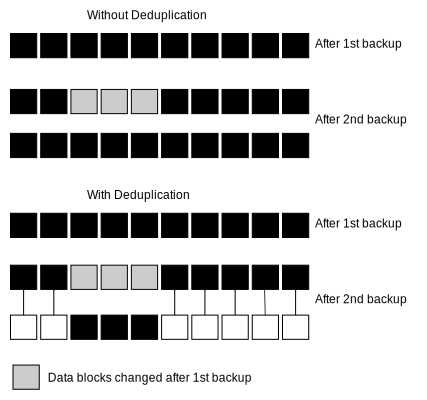
\includegraphics[width=1\columnwidth]{images/concept_dedup}
\caption{Concept of Data Deduplication}  
\end{center}
\end{figure}
Deduplication technology analyzes the incoming backup data and stores each unique block of data only once, using pointers for additional instances of the same data. When duplicate data is found, a pointer is established to the original set of data as opposed to actually storing the duplicate blocks --  removing or ``deduplicating'' the redundant blocks from the volume.

\subsection{In-line v/s Post processing}
In-line deduplication sometimes referred to as synchronous deduplication,  involve analyzing the data as it is being written. If duplicates are found, the data is not written to the disk or transmitted over the network. The advantage is that the data does not have a big landing footprint; landing footprint being amount of disk space/network bandwidth the data takes the first time it is written. However, since analyzing duplicates can be computationally intensive, this can limit the rate at which data is written to a deduplication enabled system.

Post processing or asynchronous deduplication methods attempt at duplicate elimination after data is written to the disk. Data is first written to the disk as is. It is later analyzed by a daemon process independent of the write process, to find duplicates. This daemon then modifies existing references and meta data to eliminate duplicate data. The advantage is that write speed is not hampered. However, this method has several complexities. Consider a backup of 1 GB that need to go on a disk having 700 MB space. Say after de-duplication it is reduced to 500 MB. Since its landing footprint is 1 GB, post processing based appliances cannot write this backup to this disk even though it has enough space for the compressed backup. There always has  to be provision for the maximum footprint. Other concerns include modifying the meta-data by the daemon and how it is handled for live data that may be read or written to in the midst of such a modification.

\subsection{Benefits}
Data deduplication provides a cost-effective way of packing more data on a single disk. Thus disks fill up at slower rate allowing retaining backup data on disk for longer time. Lost or corrupt files can be quickly and easily restored from backups taken over a longer time span. This makes file restores fast and easy from multiple recovery points. Efficient use of disk-space reduces the cost-per-gigabyte of storage by requiring fewer disks than in conventional backup systems. This can considerably reduce floor space and energy consumption. This leads to significant saving in operational costs. Data deduplication also makes the replication of backup data over low-bandwidth WAN links viable. Only the changed data can be sent over the network. 

Many current implementations work at the application level. This makes the deduplication technique dependant on the application. Moreover, these solutions work on structured data making them ineffective for unstructured data. 

Moving deduplication to the file system layer makes it effective even for unstructured data. This implementation is application agnostic thereby making it easier to implement it in many environments. It can work with any backup software allowing quick and cheaper deployment than application level solutions. 

\section{Tux3 Linux file system}
Tux3 is an open-source versioning file system created by Daniel Phillips \cite{4}. In broad outline, Tux3 is a conventional Unix-style inode/file/directory design with wrinkles. A Tux3 inode table is a B-tree with versioned attributes at the leaves. A file is an inode attribute that is a B-tree with versioned extents at the leaves. Directory indexes are mapped into directory file blocks as with H-Tree. Free space is mapped by a B-tree with extents at the leaves.

\begin{table}[!th]
\centering
\begin{tabular}{l | l}
Introduced on & 23rd July, 2008 \tabularnewline
\hline
Directory Contents & B-tree \tabularnewline
\hline
File Allocation & B-tree  \tabularnewline
\hline
Max file size & 2$^{60}$ bytes (1 EB) \tabularnewline
\hline
Max number of files & 2$^{48}$ \tabularnewline
\hline
Max volume size & 2$^{60}$  bytes (1 EB) \tabularnewline
\hline
Default block size & 4 KB \tabularnewline
\end{tabular}
\caption{The Tux3 Linux file system}
\label{tux3-info}
\end{table}

\begin{figure}[H]
\begin{center}
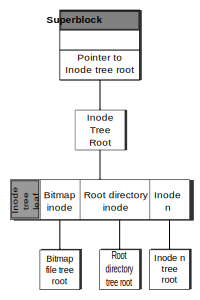
\includegraphics[width=0.7\columnwidth]{images/tux3_structure2}
\caption{Tux3 file system structure}  
\end{center}
\end{figure}

\section{Design}
The implementation of data deduplication in Tux3 does not change the file system semantics and user applications need not be aware of the underlying deduplication. The design includes an on-disk btree called Fingerprint Index and buckets which are used as locality caches.

\subsection{Fingerprints and Fingerprint Index}
The deduplication is performed at file system data block level. Unique data blocks are identified by the hash of their contents. By using a collision resistant hash function with a sufficiently large output it is possible to consider the hash of the data block as unique. Such a unique hash is called the fingerprint of a block. 

For the choice of hash function, a cryptographic hash function is chosen because it is computationally infeasible to find two distinct inputs that hash to the same value. A cryptographic hash function can also be used to ensure file system integrity. We use SHA-1 to calculate the fingerprint. 

SHA-1 is a popular hash algorithm for security systems. Assuming random hash values with a uniform distribution, a collection of \textit{n} different data blocks and a hash function that generates \textit{b} bits, the probability \textit{p} that there will be one or more collisions is bounded by the number of pairs of blocks multiplied by the probability that a given pair will collide \cite{1}
, i.e. 
$$p \leq \frac{n(n-1)}{2} \times \frac{1}{2^b}$$

Today, a large storage system may contain data in petabytes (2$^{50}$ bytes) or an exabyte (2$^{60}$ bytes) stored as 4 Kbyte blocks (2$^{48}$ blocks). Using the SHA-1 hash function, the probability of a collision is less than 2$^{-64}$ (approximately 10$^{-20}$) \cite{1}. Such a scenario seems sufficiently unlikely that we ignore it and use the SHA-1 hash as a unique identifier for a block.

The fingerprint index is a btree based data structure. A B-tree of order n is a multi-way search tree with two properties: All leaves are at the same level and the number of keys in any node lies between n and 2n, with the possible exception of the root which may have fewer keys. A btree node contains n block pointers separated by n-1 keys. 
Searching a balanced tree means that all leaves are at the same depth. There is no runaway pointer overhead. Indeed, even very large B-trees can guarantee only a small number of nodes must be retrieved to find a given key. For example, a B-tree of 10,000,000 keys with 50 keys per node never needs to retrieve more than 4 nodes to find any key. This property makes btree an ideal choice for the fingerprint index. 

The root of the fingerprint index is maintained in the file system superblock. The fingerprint btree is indexed by \texttt{hashkeys} - the first 64 bits of the SHA-1 fingerprint of the data of the block being written to the file system. It serves as a look-up structure and helps in quick and efficient detection of duplicate data blocks. Each node in the index tree contains multiple \texttt{<hashkey, block no.>} pairs where the block numbers point to nodes in the next tree level. 

\begin{figure}[H]
\begin{center}
\includegraphics[width=0.45\columnwidth]{images/fingerprint_node}
\caption{Fingerprint Index node entry}  
\end{center}
\end{figure}

The penultimate level nodes have block numbers which point to index tree leaves. The index tree leaves contain multiple triples of \texttt{<hashkey, block no. of bucket, offset>}. The \texttt{offset} is used to directly access the relevant entry rather than traversing all the bucket entries.

\begin{figure}[H]
\begin{center}
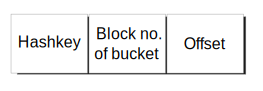
\includegraphics[width=0.7\columnwidth]{images/fingerprint_leaf}
\caption{Fingerprint Index leaf node entry}  
\end{center}
\end{figure}

\subsection{Locality Based Buckets}
As shown by previous research, data locality can be exploited to accelerating duplicate
detection process \cite{3}. A keen observation of backup data reveals that such locality exists and 
blocks tend to reappear in the same or very similar sequences across multiple backups. 

Consider a normal file composed of a hundred or more 4KB blocks. Every time that file is backed up, the same sequence of a hundred blocks will appear. If the file is modified slightly, there will be some new blocks, but the rest will appear in the same order. When new data contains a duplicate block x, there is a high probability that other blocks in its locale are duplicates of the neighbors of x. 

This observation can be used to prevent excessive disk I/O and improve performance by the introduction of the bucket abstraction. A bucket is a mapping between the SHA-1 hash values (fingerprints) and the corresponding block numbers. The buckets are filled contiguously such that the mapping of blocks belonging to the same locality are most often stored in the same bucket. The bucket entries store the entire 160 bit SHA-1 hash value.

For implementation, the in-memory inode of the files in the file system maintain two block numbers -- the \textit{current read bucket} and the \textit{current write bucket}. The current read bucket is a bucket which has a high probability of containing entries for blocks belonging to the same locality as the block being written. The current write bucket is the bucket to which the new entries of the blocks being written are made and therefore entries corresponding to neighboring blocks are together. The buckets are 4KB data blocks containing entries in the form \texttt{<fingerprint, block no., reference count>}. 

\begin{figure}[H]
\begin{center}
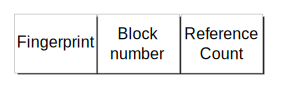
\includegraphics[width=0.7\columnwidth]{images/bucket_entry}
\caption{Entry in the bucket}  
\end{center}
\end{figure}

The reference count is incremented each time a duplicate block is detected and its reference added to the file system structure. The reference count is used to make sure that the block is not freed if it is being referred by multiple files. 
The buckets also allow for a very novel approach to manage hashkey collisions by keeping all the colliding entries together in a single `collision bucket'.

\section{Algorithm}
To implement in-line deduplication, changes need to be made to the write mechanism of the file system. The algorithm for the same is as follows -
\newpage
Input --  Buffer containing data to be written 

\begin{enumerate}
\item Compute the SHA-1 hash of the buffer data 
\item Perform a hash look-up in the current read bucket 
\item If found, 
  \begin{enumerate}
  \item[-] Do not allocate a new physical block.
  \item[-] Obtain duplicate block number from the read bucket entry.
  \item[-] Use this block number in the file's data leaf node.
  \item[-] Increment reference count of corresponding bucket entry.
  \end{enumerate}
\item Else,
  \begin{enumerate}
  \item[-] Obtain the first 64-bit of the SHA-1 fingerprint.
  \item[-] Perform look-up in the fingerprint index
  \item[-] If found,
    \begin{enumerate}
    \item Read the bucket number from the fingerprint index entry.
    \item Read the data block of the bucket into memory and make it the current read bucket.
    \item Compare the full 160-bit SHA-1 hash of the buffer with the corresponding bucket entry.
    \item If match not found, handle collision.
    \item Obtain the corresponding physical block number from the bucket entry.
    \item Use this block number in the file's data leaf node.
    \item Increment reference count of corresponding bucket entry.
    \end{enumerate}
  \item[-] Else,
    \begin{enumerate}
    \item Allocate a new physical block.
    \item Add a new entry into the fingerprint index and the current write bucket.
    \item Perform a disk write of the block.
    \end{enumerate}
  \end{enumerate}
\end{enumerate}

To elaborate the working of deduplication, consider an example scenario - \\ 
A file \textit{x} containing 10 data blocks is to be written. None of these blocks have same content as any of the existing file system blocks on disk. Hence, fingerprints of all these blocks would not match any index entry. This would result in allocation of 10 new data blocks and their corresponding entries being made into the fingerprint index and the current write bucket say \textit{b}. 
Consider another file \textit{y} resulting from appending some data to \textit{x}. Let this result into \textit{y} containing 14 data blocks of which first 10 remain same as \textit{x}. For the write of the first block, fingerprint match will be found in the index and no new physical block will be allocated. The bucket containing the corresponding entry - \textit{b} would replace the current read bucket. For the subsequent 9 duplicate blocks, the look-up would be performed only in the bucket \textit{b} which is already present in memory. This avoids the need to traverse the on-disk fingerprint index significantly reducing disk I/O. As no new physical blocks are needed for these duplicate blocks too, the deduplication mechanism will greatly improve system performance and save disk space. For the last 4 blocks for which no duplicates exist the procedure is similar to the one followed for \textit{x}. 
Thus a 14 block file \textit{y} required the allocation and disk writes of only 4 data blocks. 

\section{Performance Analysis}
Our current implementation is a part of the Tux3 FUSE (File System in Userspace) port. The figures mentioned represent the implementation of deduplication in userspace and have been computed on a Intel Core 2 Duo, T5450, 1.66GHz with 1GB 667MHz DDR2 RAM using a 10 GB partition on a Hitachi HTS54251 160 GB, 5400 rpm hard disk.

\begin{figure}[H]
\begin{center}
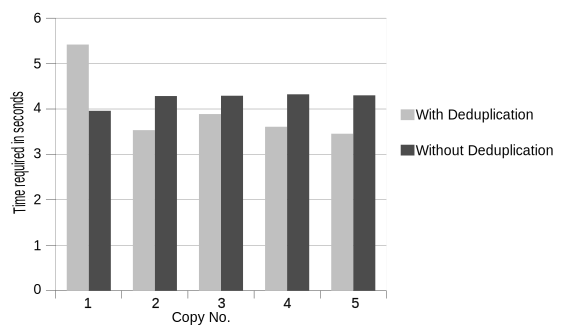
\includegraphics[width=1.1\columnwidth]{images/perf_graph}
\caption{Archival performance - Copying same file multiple times} 
\end{center}
\end{figure}
The above graph represents the timing profile for copying a 100MB video file repeatedly with and without deduplication. As observed, with deduplication enabled, the time taken for the first copy is more than that without deduplication. But for successive copies, deduplication reduces time required significantly. Thus, the Locality Based Bucket Layout enables fast duplicate detection and copying which offsets any performance hit observed in the first copy. Also, there is considerable space savings by avoiding disk blocks for the 4 duplicate copies. The above process which consumes 500MB in a normal file system, would use $\sim$ 100MB after deduplication.

\begin{table}[!th]
\centering
\begin{tabular}{| m{1.5cm} | m{1.5cm} | m{1.5cm} | m{1.5cm}|}
\hline
Database copies & Without dedup (No. of blocks allocated) & With dedup (No. of blocks allocated) & \% Saving \tabularnewline
\hline
1               & 64223                                   & 59787                                & 6.90\tabularnewline
\hline
2               & 128434                                  & 63789                                & 50.33\tabularnewline
\hline
3               & 192645                                  & 67798                                & 64.80\tabularnewline
\hline
\end{tabular}
\caption{Performance analysis using real world data}
\label{db-perf}
\end{table}

The above table shows the number of 4KB blocks required for copying the MySQL test employee database containing 3,00,024 entries with and without deduplication. The 1st copy is the original database. The 2nd copy is the database with changes to 20,000 random entries with random values. The 3rd copy is the database with 20,000 random changes over the 2nd copy. These values include the meta-data blocks along with the actual data blocks. It can be observed that there is considerable amount of space saving, approximately 50-55\% for the entire process. 

\section{Other Applications}
Besides archival storage, deduplication can be used in the following applications --
\begin{enumerate}
\item Email Servers

  In the case of an e-mail server, deduplicated storage would mean that a single copy of a message is held within its database whilst individual mailboxes access the content through a reference pointer. Apart from the benefit of reduction in disk space requirements, the primary benefit is to greatly enhance delivery efficiency of messages sent to large distribution lists. 

\item Storage systems of multimedia sharing websites

  With the advent of Web 2.0, the popularity of websites which allow multimedia sharing has grown manifold. Without content based deduplication, these websites would have to store multiple redundant copies of the same multimedia file uploaded by various users. Deduplication would remove this redundancy and allow more distinct content to be uploaded onto such servers. 
\item Common store for Virtual machine images
\end{enumerate}

\section{Advantages}

\begin{enumerate}
\item Significantly Less Storage
\item Better Performance
\item Provision for data integrity check using the fingerprint index
\end{enumerate}

\section{Conclusion}
Data deduplication technology represents one of the most significant storage enhancements in recent years. Deduplication offers the ability to store more on a given amount of storage and enables replication using low-bandwidth links, both of which improve cost effectiveness. 

In this paper, we present a block level deduplication design suitable for archival storage and backup. The btree based fingerprint index, indexes the data blocks by the fingerprints of their content. It serves as a structure for fingerprint look-up and accelerates the process of duplicate detection. The Locality Based Bucket Layout introduces the bucket abstraction which reduces excessive disk I/O and improves the deduplication performance considerably for a continuous run of duplicate blocks. Both these concepts when implemented together provide an effective and fast deduplication mechanism. 
We implement data deduplication in the btree based Tux3 file system which scales well for huge amounts of data and therefore proves to be an ideal choice for all kinds of data backups and archival storage. The in-line deduplication implementation is transparent for the system user as no changes are made to the user level semantics of duplicate files. 

Apart from backup systems data deduplication would also prove useful in applications such as email servers, storage systems of multimedia sharing websites database and file system integrity check. 

The deduplication design presented in this paper satisfies all the criteria of a good space saving solution. It does not compromise data integrity and reliability, operates seamlessly in all user environments and has minimal impact on system performance .

\section{Acknowledgements}

We wish to thank the following people for their contributions to the paper; Mr. Amey Inamdar, our mentor whose ideas and timely criticism helped us bring this to fruition. Mr. Daniel Phillips, creator Tux3, for his continued support and guidance. Prof. Rekha Kulkarni, our faculty guide at PICT. Last, but not the least, we wish to thank the anonymous reviewers, who patiently read our paper and gave us valuable inputs which helped make significant improvements in this paper.

\begin{thebibliography}{99}
\raggedright
\bibitem[1]{1} S. Quinlan, S. Dorward, 
\textit{Venti: a new approach to archival storage} (2002) [Online] Available:
\url{http://plan9.bell-labs.com/sys/doc/venti/venti.pdf}
\bibitem[2]{2} P. Kulkarni, F. Douglis, J. LaVoie, J. M. Tracey,
\textit{Redundancy Elimination Within Large Collections of Files} (2004) [Online] Available:
\url{http://www.usenix.org/event/usenix04/tech/general/full_papers/kulkarni/kulkarni.pdf}
\bibitem[3]{3} B. Zhu, K. Li, H. Patterson,
\textit{Avoiding the Disk Bottleneck in the Data Domain Deduplication File System} (2008) [Online] Available:
\url{http://www.usenix.org/event/fast08/tech/full_papers/zhu/zhu.pdf}
\bibitem[4]{4} Daniel Phillips,
\textit{The Tux3 Linux File System} (2008) [Online] Available:
\url{http://mailman.tux3.org/pipermail/tux3/2008-July/000005.html}
\end{thebibliography}
\end{document}
\end{document}

